\chapter{Component Authoring and Curation}

\section{Overview}
A key consideration underlying the design of AVM Component model, was the ability to incorporate existing model asset base which often exists in mature engineering organizations. This core feature of AVM component model, while enabling reuse of existing IP, renders it challenging to author AVM component model as the multiple domain models, developed in multiple tools, need to be wrapped and packaged together. In order to aid the engineers and developers in authoring AVM components, a component authoring framework is being developed and provided along with the META tools. 

In order to ensure quality and conformance of authored components, AVM defines a component curation process. The curation process verifies the delivered components, establishes in-class conformance of delivered components, validates the submitted component data using subject matter expertise, and hosts the submitted component on a Component Exchange infrastructure implemented by the Vehicle Forge project of AVM. The Component Exchange, similar to an online catalog, also implements services for discovery of components using a class taxonomy as well as based on component properties.


\section{Component Authoring Toolkit}
AVM Component Models incorporate metadata from their corresponding Domain Models, as well as some global properties of the component. Using this data, they describe the interfaces though which the Domain Models should be composed into a system model. They also provide structures to keep the parameters of each Domain Model synchronized.

To support the creation and maintenance of these structures within AVM Component Models, a Component Authoring Toolkit is provided with the OpenMETA CyPhy tools.

The framework addresses the following two primary use-cases:
\begin{enumerate}
\item{Creating a New Component Class}
\item{Creating a New Instance of an Existing Component Class}
\end{enumerate}

Figure \ref{Authoring_workflow_1} depicts the workflow involved in authoring a new component class focusing on CAD domain model. The component authoring is initiated from the OpenMETA CyPhy tools. Subsequently, the author launches the CAD authoring tool (PTC Creo Parametric) using the META-Link capability of OpenMETA Tools. This enables the author to automatically construct domain model ports and CAD parameters in the OpenMETA CyPhy environment. Once the component ports are created, the author can invoke the Component Authoring tool from OpenMETA, and package additional artifacts required for the component and created the complete component package. The authoring tool also includes component validation tools (described later) that can be used to validate the authored components. Additionally, the authoring tool also provides capability to automatically submit the authored component for curation through the Vehicle Forge portal. 

\begin{figure}
\includegraphics*[width=\textwidth]{Authoring_workflow_1}
\caption{Component Authoring Workflow (New Component Class)}
\label{Authoring_workflow_1}
\end{figure} 

Figure \ref{Authoring_workflow_2} depicts a similar workflow for authoring a new instance of an existing component class. In this second use case parameterized templates and domain models already exist for the component class, and the component author needs to instantiate parameter values for their specific component instance. When parametric domain models are not available, as often the case with discrete CAD models, the author must create the domain model wrapper for the CAD model using the META-Link and CAD authoring tool (PTC/Creo parametric currently)


\begin{figure}
\includegraphics*[width=\textwidth]{Authoring_workflow_2}
\caption{Component Authoring Workflow (New Component Instance)}
\label{Authoring_workflow_2}
\end{figure} 


In support of these use cases, the Component Authoring Toolkit includes modules for common tasks, such as:
\begin{itemize}
\item{Load a component model template and allow users to edit parameters}
\item{Import metadata from a class in a Modelica library (parameters, connectors)}
\item{Import metadata from a Creo part or assembly (parameters, datums)}
\end{itemize}

Additional details on the Component Authoring Toolsuite, are included in the OpenMETA CyPhy documentation.

\section{Curation Workflow}
Component authors can submit components for curation using the Vehicle Forge portal. The curation workflow verifies the component and checks the in-class conformance of a given component. Optionally, the curation workflow can also validate the component with the involvement of subject matter experts. During submission the component author can define the distribution parameters and restriction of the submitted component, depending on which the component is repositoried in the global component exchange or a local component exchange. 

\begin{figure}
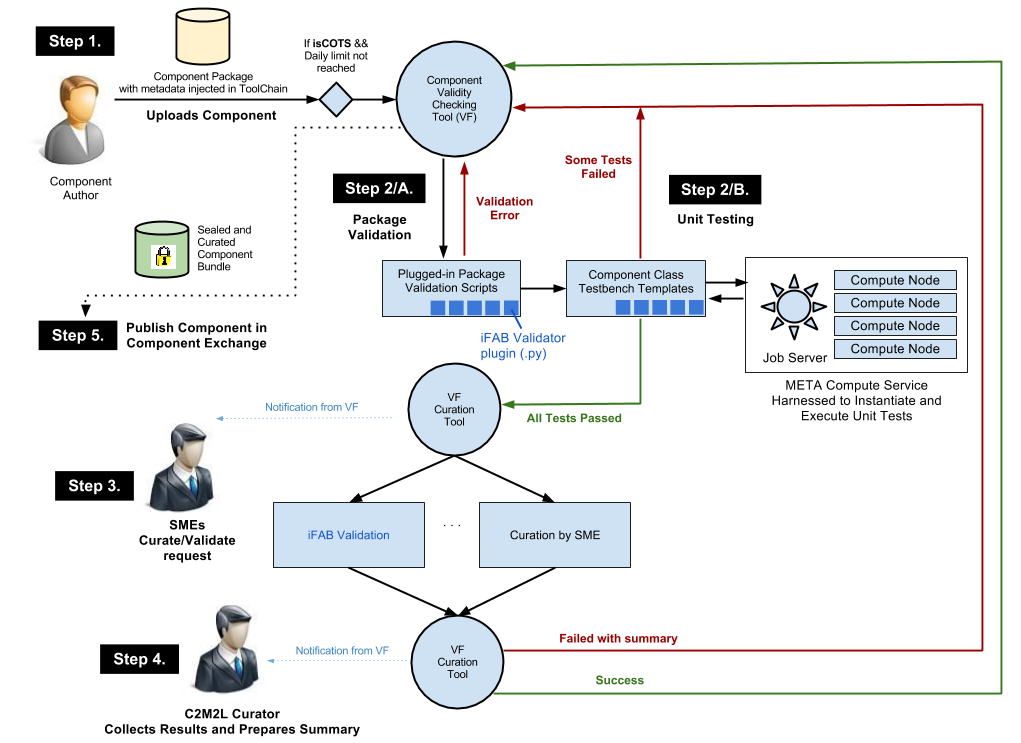
\includegraphics[width=\textwidth]{Curation_Workflow}
\caption{Component Curation Workflow}
\label{Curation_Workflow}
\end{figure}

\section{Component Model APIs}
See \textit{\autoref{ACMAPI}: \nameref{ACMAPI}}.

\section{Component Model Taxonomy}
